\chapter{研究内容}\label{ux7814ux7a76ux5185ux5bb9}

\section{optparseとThorの比較}\label{}

\subsection{optparse}\label{optparse}

今回の研究対象のmy\_helpは,optparseで実装されている.optparseはrubyの標準ライブラリであり,rubyでコマンドラインのオプションを操作するためのライブラリである\cite{opt1}.optparseが操作するオプションは,下記のonメソッドで設定する.

\begin{screen}
{\small
\begin{verbatim}
def execute
  @argv << ’--help’ if @argv.size==0
  command_parser = OptionParser.new do |opt|
    opt.on(’-v’, ’--version’,’show program Version.’ ) { |v|
      opt.version = MyHelp::VERSION
      puts opt.ver
    }
    opt.on(’-l’, ’--list’, ’list specific helps’){list_helps}
    #中略
  end
  #中略
end
    
def list_helps
#中略
end
#後略
\end{verbatim}}
\end{screen} 


上記のコードはoptparse版my\_helpの一部である.第1引数はショートオプションで,-aや-dのような形で設定する.同様にして,第2引数はロングオプションを表し,-\/-addや-\/-deleteのように,第3引数はそのオプションの説明文で,helpで表示される説明文を設定する.後ろのブロックには,そのオプションが指定された場合に実行されるコードを記述する
\cite{opt2}.しかしこのライブラリでは自然言語に近い,ハイフンなしのサブコマンドを実装するには相当な書き換えが必要となる.

メソッドの引数でオプションを定義し,引数が指定された時の処理をブロックで記述する.ブロックの引数にはオプションが指定されたことを示すtrueが渡される.onメソッドが呼ばれた時点ではオプションは実行されず,定義されるだけである.parseが呼ばれた際,コマンドラインにオプションが登録されていれば実行される.

オプション定義の際,スペースの後に任意の文字を追加すると,そのオプションは引数を受け取るオプションになる.その文字に{[}{]}をつけることで引数は必須でなくなる.また引数がハイフンで始まる場合,オプションとの間にハイフンを2つ挟むことで引数として認識される.

helpとversionのサブコマンドはデフォルトで作成される.

\subsection{Thor}\label{thor}

本研究ではoptparseの代わりのライブラリとしてThorの採用を検討する.Thorは,コマンドラインツールの作成を支援するライブラリであり,gitやbundlerのようにサブコマンドを含むコマンドラインツールを簡単に作成することができる
\cite{koichiro}.Thorには以下のような特徴がある.

1.コマンドラインオプションのパーズやサブコマンドごとのヘルプを作るなどの面倒な作業を簡単にこなすことができ,手早くビルドツールや実行可能なコマンドを作成できる
\cite{hibariya}.

2. 特殊なDSL(Domain Specific
Language)を使わずにメソッドを定義することで処理を記述するため,テストを行いやすい
\cite{hibariya}.

3.optparseでは作成することが困難な,マイナスを伴わない(自然言語に近い)サブコマンドを実装することが可能である.下記はThor版my\_helpの一部である.

\begin{screen}
{\small
\begin{verbatim}
desc 'list, --list', 'list specific helps'
    map "--list" => "list"
    def list
      print "Specific help file:\n"
      local_help_entries.each{|file|
        file_path=File.join(@local_help_dir,file)
        help = YAML.load(File.read(file_path))
        print "  #{file}\t:#{help[:head][0]}\n"
      }
    end
end
\end{verbatim}}
\end{screen}


optparseではonメソッドでコマンドの登録を行い,その後のdefでコマンドの振る舞いを定義している.それに対してThorは登録と定義を同時に行うことが可能である.また,Thorを継承したクラスのパブリックメソッドがそのままコマンドになるので非常に簡単にコマンドを作成することが可能である.Thorはコマンドを作成した時点で自動的にヘルプを生成し,コマンドを指定せずにコマンドラインアプリを実行するとヘルプを表示する.

\begin{table}[H]
\centering
\begin{center}
\caption{optparse とThor の比較. \label{opt_thor}}
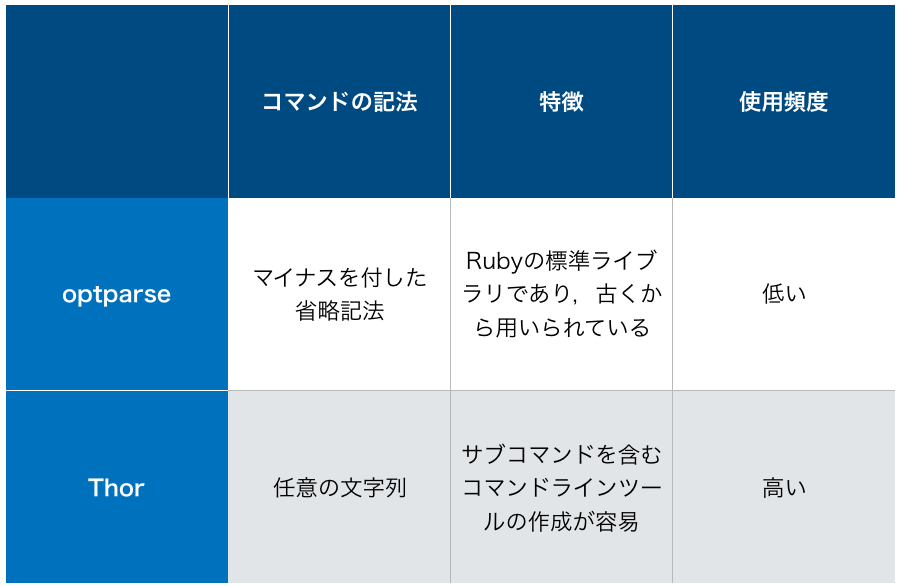
\includegraphics[width=150mm]{../.././figs/opt_thor.png}
\end{center}


\label{fig:This}
\end{table}

\subsection{比較}\label{}

書き換えの前に,単純なCLIを例にoptparseとThorの比較を行った.今回はコマンドに続けてnameを入力すると,Hello nameと出力するCLIをoptparseとThor,それぞれを用いて作成し,コード量や使用感を比較する.1つめのソースコードがoptparseを用いたもの(optparse.rb),2つめのソースコードがThorを用いたもの(thor.rb)である.

\begin{screen}
{\small
\begin{verbatim}

options = {:name => nil}

parser = OptionParser.new do|opts|
  opts.on('-n', '--name name', 'Give your own name') do |name|
    options[:name] = name;
    end

  opts.on('-h', '--help', 'Displays Help') do
    puts opts
    exit
    end
end

parser.parse!

sayHello = 'Hello ' + options[:name]

puts sayHello

\end{verbatim}}
\end{screen}

\begin{screen}
{\small
\begin{verbatim}

require 'thor'

class MyCLI < Thor
  desc "hello NAME", "say hello to NAME"
  def hello(name)
    puts "Hello #{name}"
  end
end

MyCLI.start(ARGV)

\end{verbatim}}
\end{screen}

optparse.rbは,onメソッドで,入力された名前を受け取る-nというコマンドの定義を行い,parser.parse!以降でHello nameと出力するように記述を行った.また,-hのコマンドでヘルプを表示できるようにコマンドを登録した.本来ならば,-nではなく-h(helloの頭文字)で登録したかったのだが,ヘルプを表示するコマンドが-hであり,重複してしまうためやむを得ず-nとした.一方thor.rbでは,Thorを継承したクラスの中でnameの受け取りとHello nameの表示を行うようにhelloコマンドを設定した.optparseと違い,Thorでは自動でヘルプが作成されるため,helpコマンドは作成していない.optparse.rbはサブコマンドを書かずに実行すると,エラーになってしまうが,thor.rbではコマンド一覧を表示してくれる.

コード量は,helpを自動で生成する分,thor.rbの方が短くなっており,descの中で一つのコマンドが完結しているということもあってoptparse.rbよりも書きやすく感じられた.また,実際にコマンドを入力する際,thor.rbの方が自然言語に近いコマンドのため直感的に入力することができた.さらに,thor.rbでhelloの後にname(引数)を入力せずに実行するとhelloコマンドのusageが表示されるなど,使用感はthor.rbの方がよく感じられた.

    \section{Thor化に伴う書き換え(具体的な作業)}\label{thorux5316ux306bux4f34ux3046ux66f8ux304dux63dbux3048ux5177ux4f53ux7684ux306aux4f5cux696d}

optparseからThorへの書き換えの際,第一に必要となるのは,\textasciitilde{}.gemspecファイル内にThorがインストールされるように変更を加えることである.

\begin{verbatim}
spec.add_development_dependency "thor"
\end{verbatim}

この記述は,作成しているコマンドラインツールがThorに依存性を持つことを意味している.optparseで書いた場合は,Thorに依存性を持つ必要がなく,当然このような記述はされていないので,上の一文を書き加える必要がある.また,bundle
updateをターミナル上で実行することで,ローカルでのコマンドラインツールを実行した際にThorが適用されるようにアップデートされる.そうすることで,Thorの記述が実際にソースファイルで使用できるようになる.

\section{Thorによるサブコマンド}\label{thorux306bux3088ux308bux30b5ux30d6ux30b3ux30deux30f3ux30c9}

次に,コマンドが呼ばれる流れについて説明する.

\begin{enumerate}
\def\labelenumi{\arabic{enumi}.}
\tightlist
\item
  コマンドを実行する.
\item
  コマンドを実行すると,exeディレクトリの中にあるコマンド名と同じ名前のファイル(以降コマンドファイルと呼ぶ)が実行される.
\item
  コマンドファイル内でlibディレクトリ内のソースファイルをrequireしておき,クラス内のコマンドを解析する関数を呼び出す.
\item
  ソースファイル内に書かれた処理が実行される.
\end{enumerate}

このような流れでコマンドが呼び出され,処理が行われる.Thorとoptpaseの差異は4.におけるコマンドの解析による処理関数への中継の方法である.

\section{exeディレクトリの書き換え}\label{exeux30c7ux30a3ux30ecux30afux30c8ux30eaux306eux66f8ux304dux63dbux3048}

exeディレクトリの中にあるコマンドファイルについて書き換えを行う.まずはoptparseを使用した際のコマンドファイルの記述を記載する.

\begin{screen}
{\small
\begin{verbatim}
!/usr/bin/env ruby                                                                                                               
require "my_help_opt"

MyHelp::Command.run(ARGV)
\end{verbatim}}
\end{screen}

optparseの場合,MyHelp::Command.run(ARGV)というクラス関数を実行することでコマンドを呼び出している.しかし,Thorはoptparseのようにrun(ARGV)を用いず,start(ARGV)というクラス関数を実行してコマンドを呼び出す.よって,runをstartに書き換える作業が必要になる.以下にThorを使用した際のコマンドファイルの記述を記載する.

\begin{screen}
{\small
\begin{verbatim}
!/usr/bin/env ruby                                                                                                               
require "my_help_thor"

MyHelp::Command.start(ARGV)
\end{verbatim}}
\end{screen}

\section{libディレクトリ}\label{libux30c7ux30a3ux30ecux30afux30c8ux30ea}

まず,self.runについてであるが,Thorでは使用されないのでこの一文は削除する.次にinitializeであるが,こちらについては変更が必要である.そもそもinitializeとはmy\_helpを動かすのに必要なディレクトリがあるかどうかを調べるメソッドであり,なければここで作ることができる.optparseのinitializeではargv={[}{]}となっているところをThorでは(アスタリスク)argvとする必要がある.また,大きな違いはsuperの有無である.optparseではsuperは必要ないのだが,Thorでは必要になる.

\section{その他オプション}\label{ux305dux306eux4ed6ux30aaux30d7ux30b7ux30e7ux30f3}

optparseではコマンド実行の際,引数の解析を行い,その引数に合わせた関数を呼び出す,という手順で動作している.その手順を記述した関数がexecuteである.


\begin{screen}
{\small
\begin{verbatim}
def execute
      @argv << '--help' if @argv.size==0
      command_parser = OptionParser.new do |opt|
        opt.on('-v', '--version','show program Version.') { |v|
          opt.version = MyHelp::VERSION
          puts opt.ver
        }
        
        opt.on('-l', '--list', 'list specific helps'){list_helps}
        opt.on('-e NAME', '--edit NAME',
         'edit NAME help(eg test_help)'){|file| edit_help(file)}
        opt.on('-i NAME', '--init NAME',
         'initialize NAME help(eg test_help).'){|file| init_help(file)}
        opt.on('-m', '--make', 'make executables for all helps.'){make_help}
        opt.on('-c', '--clean', 'clean up exe dir.'){clean_exe}
        opt.on('--install_local','install local after edit helps')
        {install_local}
        opt.on('--delete NAME','delete NAME help'){|file| delete_help(file)}
      end
      
      begin
        command_parser.parse!(@argv)
      rescue=> eval
        p eval
      end
      exit
end
\end{verbatim}}
\end{screen}

しかしThorの場合,executeのような間を取り持つ関数を用意する必要がなく,関数自体をコマンドとして登録していく形をとっているので,この関数は不必要である.以下にThorでの関数宣言を記載する.optparseno場合,-iというコマンドで呼び出されている処理をinitというコマンドで呼び出されるように書き換えたのが以下の関数である.


\begin{screen}
{\small
\begin{verbatim}
desc 'init NAME, --init NAME', 'initialize NAME help(eg test_help).'
 # 関数についての説明,ここがヘルプで表示される.
map "--init" => "init"
 --オプションでも呼び出すことが可能.
def init(file)
以下は変更なし
    p target_help=File.join(@local_help_dir,file)
    if File::exists?(target_help)
        puts "File exists. rm it first to initialize it."
        exit
    end
    p template = File.join(@default_help_dir,'template_help')
    FileUtils::Verbose.cp(template,target_help)
end
\end{verbatim}}
\end{screen}

このように書き換えることで,Thorを使用したオプションの設定を行うことができるのだが,実際に動かしてみるとエラーが表示されることがある.ここで表示されるエラーは,コマンドとして設定されていない関数があることについての警告文である.その関数はコマンドとして使用しないということを明確に記述することでこの警告を消すことが可能である.

\begin{screen}
{\small
\begin{verbatim}
no_commands do

    この間にコマンド設定しない関数を記述

end
\end{verbatim}}
\end{screen}

\section{変更後のオプション}\label{}

オプションを省略記法から自然言語に近い記法に変更したことでより直感的なコマンド入力が可能になると思われる.以下にThorで書き換えた後のmy\_helpのオプション一覧を示す.

\begin{screen}
{\small
\begin{verbatim}
Commands:
my\_help clean, -\/-clean clean up exe dir.
my\_help delete NAME, -\/-delete NAME delete NAME help
my\_help edit NAME, -\/-edit NAME edit NAME help(eg test\_help)
my\_help help {[}COMMAND{]} Describe available commands or one specific
command
my\_help init NAME, -\/-init NAME initialize NAME help(eg test\_help).
my\_help install\_local, -\/-install\_local install local after edit
helps
my\_help list, -\/-list list specific helps
my\_help make, -\/-make make executables for all helps.
my\_help version, -v show program version
\end{verbatim}}
\end{screen}
    